\documentclass[preprint, 3p,
authoryear]{elsarticle} %review=doublespace preprint=single 5p=2 column
%%% Begin My package additions %%%%%%%%%%%%%%%%%%%

\usepackage[hyphens]{url}

  \journal{Computers \& Education} % Sets Journal name

\usepackage{graphicx}
%%%%%%%%%%%%%%%% end my additions to header

\usepackage[T1]{fontenc}
\usepackage{lmodern}
\usepackage{amssymb,amsmath}
% TODO: Currently lineno needs to be loaded after amsmath because of conflict
% https://github.com/latex-lineno/lineno/issues/5
\usepackage{lineno} % add
\usepackage{ifxetex,ifluatex}
\usepackage{fixltx2e} % provides \textsubscript
% use upquote if available, for straight quotes in verbatim environments
\IfFileExists{upquote.sty}{\usepackage{upquote}}{}
\ifnum 0\ifxetex 1\fi\ifluatex 1\fi=0 % if pdftex
  \usepackage[utf8]{inputenc}
\else % if luatex or xelatex
  \usepackage{fontspec}
  \ifxetex
    \usepackage{xltxtra,xunicode}
  \fi
  \defaultfontfeatures{Mapping=tex-text,Scale=MatchLowercase}
  \newcommand{\euro}{€}
\fi
% use microtype if available
\IfFileExists{microtype.sty}{\usepackage{microtype}}{}
\usepackage[]{natbib}
\bibliographystyle{plainnat}

\ifxetex
  \usepackage[setpagesize=false, % page size defined by xetex
              unicode=false, % unicode breaks when used with xetex
              xetex]{hyperref}
\else
  \usepackage[unicode=true]{hyperref}
\fi
\hypersetup{breaklinks=true,
            bookmarks=true,
            pdfauthor={},
            pdftitle={From heartbeat to data -- Using wearable fitness trackers as an affordable approach to assess teacher stress},
            colorlinks=false,
            urlcolor=blue,
            linkcolor=magenta,
            pdfborder={0 0 0}}

\setcounter{secnumdepth}{5}
% Pandoc toggle for numbering sections (defaults to be off)


% tightlist command for lists without linebreak
\providecommand{\tightlist}{%
  \setlength{\itemsep}{0pt}\setlength{\parskip}{0pt}}




\usepackage{tabularx}
\usepackage{threeparttable}
\usepackage{booktabs}
\usepackage{array}
\usepackage{caption}
\usepackage{tablefootnote}
\usepackage{float}
\usepackage{wrapfig}
\usepackage{pdflscape}
\usepackage{longtable}



\begin{document}


\begin{frontmatter}

  \title{From heartbeat to data -- Using wearable fitness trackers as an
affordable approach to assess teacher stress}
    \author[Leipzig University]{Mandy Klatt%
  \corref{cor1}%
  \fnref{1}}
   \ead{mandy.klatt@uni-leipzig.de} 
    \author[Leipzig University]{Peer Keßler%
  %
  \fnref{2}}
   \ead{Peer@example.com} 
    \author[Leipzig University, Max Planck Institute for Evolutionary
Anthropology]{Gregor Kachel%
  %
  \fnref{1}}
   \ead{gregor@example.com} 
    \author[Leipzig University]{Christin Lotz%
  %
  \fnref{1}}
   \ead{christin@example.com} 
    \author[Leipzig University]{Anne Deiglmayr%
  %
  \fnref{3}}
   \ead{anne@example.com} 
      \affiliation[Leipzig University]{
    organization={Empirische Schul- und
Unterrichtsforschung},addressline={Marschnerstr.
29},city={Leipzig},postcode={4109},state={Sachsen},country={Germany},}
    \affiliation[Max Planck Institute for Evolutionary Anthropology]{
    organization={Department},addressline={Deutscher Pl.
6},city={Leipzig},postcode={4103},state={Sachsen},country={Germany},}
    \cortext[cor1]{Corresponding author}
    \fntext[1]{ConceptualizationWriting - Original Draft
PreparationWriting - Review \& Editing}
    \fntext[2]{Writing - Original Draft PreparationWriting - Review \&
Editing}
    \fntext[3]{Supervision}
  
  \begin{abstract}
  Past research on physiological indicators of teacher stress often had
  to rely on expensive and obtrusive assessment methods. Modern fitness
  trackers represent a non-invasive and convenient alternative. This
  study investigated the use of wrist-worn fitness trackers to assess
  teacher heart rate (HR) as an indicator of stress during teaching. In
  a laboratory study, we used a Fitbit® fitness tracker to assess
  teachers´ HR before, during, and after a potentially stressful
  micro-teaching session. Our results demonstrate that the fitness
  tracker was indeed useful for mapping teachers' stress, with the data
  showing how teachers' HR increased before, peaked during, and
  progressively decreased after the micro-teaching session. Moreover, we
  related the fitness tracker data to retrospective teacher
  self-reports. We found that teachers' subjective stress appraisals,
  together with their teaching experience, explained only small amounts
  of variance in HR data. We discuss the potential of fitness trackers
  as an affordable and ubiquitous assessment tool for research on
  teacher stress in the classroom and provide advice for practical
  implementation.
  \end{abstract}
    \begin{keyword}
    teacher stress \sep fitness tracker \sep heart rate \sep classroom
disruptions \sep wearable technology \sep 
    physiological stress measurement
  \end{keyword}
  
 \end{frontmatter}

\section{Introduction}\label{introduction}

The teaching profession is one of the most stressful professions, with
teachers facing a host of stressors during their everyday work
\citep{smith2000, herman2020, schult2014belastet}. To better understand
mechanisms in teacher stress, there is a growing research interest in
physiological measures such as heart rate (HR) as online measures of
teachers' stress during teaching
\citep{karner2021teachers, wettstein2020ambulatory}. For example, it has
been shown that teacher-centered activities and typical
classroom-related stressors increase teacher HR during teaching
activities
\citep{sperka1995, scheuch1997psychophysische, donker2018, junker2021, huang2022class}.
However, previous studies have often relied on expensive and obtrusive
electrocardiographs (ECG). Modern fitness trackers represent a
non-invasive and convenient alternative. \citep{ferguson2015}

Classroom disruptions are a major stressor in teachers' daily work
\citep{boyle1995structural, aloe2014multivariate}, and learning how to
deal with them is an important aspect of professional expertise
\citep{wolff2015keeping}. According to \citet{lazarus1990theory}
transactional model of stress and coping, the experience of stress in
response to stressors such as classroom disruptions depends on the
teacher´s subjective appraisal, which, in turn, depends on their coping
resources, such as their professional knowledge. The resulting stress
response has a psychological, physiological, or behavioral dimension
\citep{kyriacou1978}. Therefore, in order to better understand how
classroom stressors affect teachers' stress response, subjective
self-reports should be accompanied by objective, physiological measures
\citep{wettstein2021}. Teachers' use of wrist-worn fitness trackers in
educational research provides fine-grained, in vivo data, allowing
researchers as well as teachers themselves to monitor their
physiological stress response continuously during teaching, across
settings, and at low costs. Being able to monitor, and eventually
counteract, teacher stress levels appears particularly relevant given
the profession's generally high stress levels and associated negative
health effects \citep{johnson2005experience, montgomery2005meta}. To
harness this potential, the present study explored the use of
wrist-based fitness trackers as a tool to assess teachers' HR, as an
indicator of stress, before, during, and after a teaching session during
which typical, potentially stressful, classroom disruptions occurred.
Further, we explored to what extent teachers' subjective appraisals of
classroom disruptions and their teaching experience predicted teacher
stress as assessed by the fitness tracker.

\subsection{Fitness trackers as a ubiquitous, low-cost tool for
assessing physiological stress
responses}\label{fitness-trackers-as-a-ubiquitous-low-cost-tool-for-assessing-physiological-stress-responses}

Fitness trackers provide data on physical activity and cardiovascular
parameters such as HR, supporting personalized fitness goals
\citep{nuss2021effects} and stress management \citep{hao2018chrv}. They
can be used as ubiquitous, low-cost, and unintrusive data collection
instruments \citep{godfrey2018z}, and their wide-spread use and everyday
availability align with the increasing popularity and acceptance of
wearables among the general population \citep{peng2022acceptance}. In
contrast to self-reported questionnaires on stress
\citep{chaplain2008, liu2020} that are prone to biases like social
desirability \citep{razavi2001self} or recall errors
\citep{van2016accuracy}, fitness trackers, as ambulatory assessment
methods \citep{trull2013ambulatory, wettstein2020ambulatory}, offer more
objective insights into teachers' stress levels by monitoring teachers'
physiological stress responses without disrupting teaching
\citep{donker2018, runge2020}.

One important health parameter assessed by nearly all wrist-worn fitness
trackers is heart rate \citep{scalise2018wearables}. HR indicates the
number of heartbeats within one minute and is typically expressed as
beats per minute (BPM)
\citep{berntson2007cardiovascular, hottenrott2007}. At rest, the average
HR of adults typically ranges between 60 and 80 BPM
\citep{sammito2015guideline}. HR can be detected and measured in
different ways using sensors, such as electrocardiography (ECG) or
photoplethysmography (PPG) \citep{mukhopadhyay2017wearable}. While ECG
sensors offer precise measurements by detecting the heart's electrical
activity, their intrusive nature and requirement of direct skin contact
may limit their suitability \citep{kranjec2014non}, particularly in
educational settings. In contrast, photoplethysmography (PPG) is a
rather uncomplicated and inexpensive technique to measure HR, commonly
found in commercially available fitness trackers
\citep{castaneda2018review}. This optical method assesses HR by flashing
green or red lights to measure changes in blood volume in the
capillaries of the skin \citep{allen2007photoplethysmography}.

Physiologically, HR is regulated by the sympathetic and parasympathetic
nervous systems \citep{pham2021}. An increase in sympathetic activity
results in HR being sped up (``fight or flight'' response)
\citep{taelman2009influence}; whereas an increase in parasympathetic
activity results in HR being slowed down (``rest and digest'' response)
\citep{battipaglia2015}. Stress or mental and physical strain directly
increases HR \citep{custodis2014heart, sachs2014}. Therefore, an
increase in HR can be regarded as an indicator of increasing stress, and
a decrease as an indicator of relaxation and ease \citep{kyriacou1978}.
Thus, fitness trackers offer low-cost and unobtrusive access to
psychological stress data.

\subsection{HR in teaching-learning
contexts}\label{hr-in-teaching-learning-contexts}

Prior research, typically using ECG methods, has shown that changes in
teachers' HR can be mapped onto stressors they experience during
teaching. For example, teachers' HR tends to increase when teachers take
an exposed position in student-teacher interaction
\citep{sperka1995, scheuch1997psychophysische, donker2018, junker2021}.
\citet{sperka1995} for example recorded the HR of 16 pre-service
teachers during their first lesson and showed that teachers' HR
increased significantly during teaching. The activation was particularly
prominent at the beginning of the lesson and decreased over the course
of the lesson. The authors suggested that pre-service teachers'
proactive coping strategies, such as actively managing student
interactions, helped lower their HR levels. Other ECG studies identified
typical stressors predicting increases in HR, such as class size
\citep{huang2022class}, or low student engagement and motivation
\citep{junker2021}. \citet{junker2021} recorded the HR of 40 teachers
during a real classroom lesson. Again, teacher stress, induced by
factors such as low student engagement (e.g., lack of motivation or
interest in tasks) or teacher-centered activities (e.g., teacher-focused
classroom activities), resulted in elevated HR.

More recent studies have begun using wrist-worn fitness trackers to
investigate HR trends in instructional settings
\citep{Darnell2019, chalmers2021}. \citet{Darnell2019} measured the HR
of 15 medical college students listening to lectures, using wrist-worn
devices. The analysis revealed a constant decrease in HR throughout the
lecture, with HR peaks during more interactive learning phases.
\citet{chalmers2021} used HR data from a fitness tracker to identify
physiological changes during stress-inducing tasks (i.e., the Trier
Social Stress Test; \citet{kirschbaum1993trier}{]}. Average HR increased
significantly from the resting to the stress inducing phases. Even
though the participants of these previous studies
\citep{Darnell2019, chalmers2021} were not teachers but learners, the
results are relevant for studying teacher stress as they demonstrated
that HR can be effectively recorded using fitness trackers over the
course of a whole learning unit, and HR changes are in line with the
occurrence of activating or stress-inducing tasks.

To the best of our knowledge, only one study has directly assessed
teachers' HR during teaching using a wrist-worn fitness tracker:
\citet{runge2020} assessed HR as an indicator of stress in four
in-service teachers during authentic lessons. They used fitness
trackers' recordings to create a profile for each teacher, with the aim
of differentiating between teachers reporting higher vs.~lower levels of
stress. It was found that the combination of a high HR, a high number of
steps, and short sleep duration was characteristic for teachers
reporting high stress levels. However, it should be noted that the
generalizability of these results is limited due to the small sample
size.

In summary, previous studies have revealed that teachers' (and
students') HR changes depend on their activities and the stressors they
experience, with an increase in HR already before the expected stressors
occur, and with peaks in activating phases
\citep{Darnell2019, chalmers2021}. For teachers, teacher-centered phases
led to an increase in HR
\citep{sperka1995, scheuch1997psychophysische, donker2018, junker2021}.
However, there is a lack of studies using teacher-worn fitness trackers
in larger samples, exploring the feasibility of this convenient tool for
researching links between teachers' HR and stress inducing events and
mechanisms.

\subsection{A model of teacher stress}\label{a-model-of-teacher-stress}

According to \citet{kyriacou1978}, teacher stress can be defined as a
negative affective response, typically accompanied by physiological
changes such as increased HR, triggered by job-related demands, and
perceived as threatening to one's self-esteem or well-being. Coping
mechanisms help to reduce the perceived threat. Kyriacou's definition of
teacher stress (see \citet{kyriacou1978} and, for a more recent
adaptation, \citet{van2006stress}) is based on the transactional stress
model by Lazarus and colleagues {[}lazarus1966psychological;
\citet{lazarus1990theory}{]}, which highlights the interaction between
an individual and the environment, whereby stress refers to a person's
subjective reaction to an event (a stressor) that exceeds the person's
adaptive resources.

\begin{figure}[htbp]
  \centering
  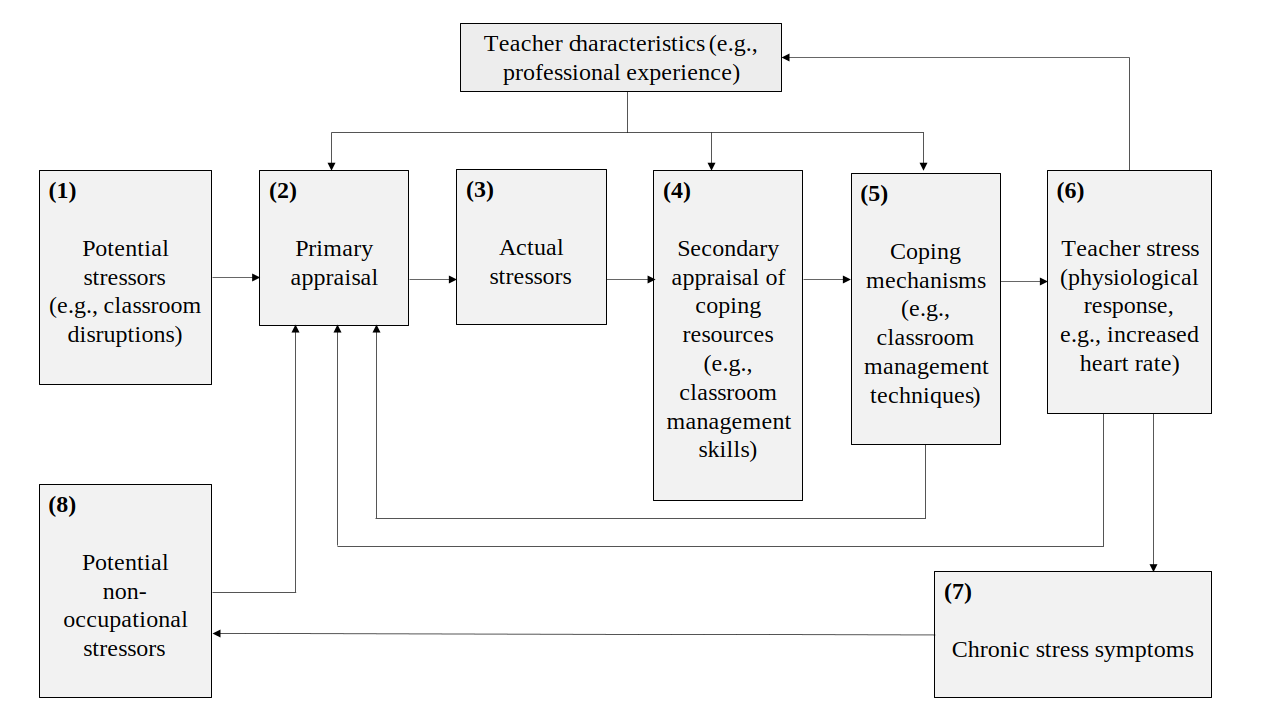
\includegraphics[width=1\textwidth]{images/Model_Teacher_Stress_adapted_new.pdf}
  \caption{A model of teacher stress (adapted from van Dick 2006, p.37, modified by the authors)}
  \label{A model of teacher stress (adapted from van Dick 2006, p.37, modified by the authors)}
\end{figure}

Fig. 1 shows, in a simplified way, how classroom events affect teachers'
stress level, according to the adaptation of the Lazarus model to
teacher stress proposed by \citet{van2006stress}: When potential
stressors (e.g., classroom disruptions) occur during teaching (1),
teachers intuitively judge how disruptive the event is in a primary
appraisal (2). If potential stressors are judged as threatening, i.e.,
as actual stressors (3), teachers consider whether they have sufficient
resources for coping with the stressors (4). Teachers utilize these
resources in trying to cope with the stressors, e.g., by employing
classroom management strategies (5). In cases when coping fails, stress
ensues, often accompanied by physiological reactions like increased HR
(6). As part of the coping process, and dependent on its outcomes,
teachers re-evaluate the stressor (7).

As shown in Fig. 1, teachers' primary and secondary appraisal as well as
coping attempts are influenced by professional experience. As
professional experience grows, teachers develop cognitive scripts for
managing classroom events, resulting in more complex and problem-focused
classroom management skills \citep{wolff2021classroom}, and thus more
effective coping and less stress. Empirically, classroom management
skills and problem-focused coping styles are linked to fewer instances
of emotional exhaustion \citep{maslach2001job, clunies2008self}. Novices
in the teaching profession, on the other hand, face considerable stress
and often feel overwhelmed by the demands of teaching
\citep{ophardt2017klassenmanagement, wolff2015keeping, klusmann2012berufliche}
with many leaving the profession within the first five years
\citep{ingersoll2003}. Accordingly, when resources are lacking and
coping fails, negative consequences for health (e.g., burnout) and for
work (e.g., high turnover rates) can arise
\citep{jalongo2006, unterbrink2007, aloe2014multivariate}, highlighting
the importance of professional expertise for managing teacher stress
\citep{fisher2011}.

\subsection{Present Study}\label{present-study}

The present study aimed to explore the relations between teachers' HR
response, and their subjective appraisals of stress during a
micro-teaching unit, and to relate their self-reported appraisals and
physiological stress responses to their teaching experience. We analyzed
data from in-service and pre-service teachers who participated in a
laboratory study as part of a larger project targeting the development
of classroom management skills. Participants came to the lab
individually and taught a short lesson to a class of three actors (i.e.,
trained student assistants) who performed several typical and possibly
disruptive classroom events. The micro-teaching unit was thus
potentially stressful for the participants. The aims of the present
study were twofold:

\begin{enumerate}
\def\labelenumi{(\arabic{enumi})}
\tightlist
\item
  The first research goal was to investigate whether HR measures
  assessed by a wrist-based fitness tracker were a suitable and
  effective method for mapping teachers' HR over the course of the lab
  study, with a total duration of approximately 2 hours, including
  phases before, during, and after the stressful micro-teaching unit.
\end{enumerate}

Looking at HR measures globally, we expected the participants to show an
initial increase in their HR, followed by a peak during the
micro-teaching unit and a decrease for the remaining phases. In
addition, we examined whether z-standardization of the participants' HR
could serve as a useful method to account for individual differences in
baseline HR: We expected to observe the same trends in both standardized
and non-standardized HR values.

In addition, we selected five representative 10-minute intervals from
the five phases of the lab study (see Figure 2) in order to test the
hypotheses that, regarding HR levels, teachers' HR would be the highest
during the micro-teaching unit, compared to all other phases
(\textbf{Hypothesis 1a}), and, regarding HR slopes, that teachers' HR
would increase while they were preparing for teaching (pre-teaching
interval), but decrease in all of the following intervals, i.e.~when
they were habituating to and recovering from the stressful
micro-teaching unit (\textbf{Hypothesis 1b}).

\begin{enumerate}
\def\labelenumi{(\arabic{enumi})}
\setcounter{enumi}{1}
\tightlist
\item
  We further explored whether teaching experience made a difference in
  how teachers' HR reacted to the classroom disruptions. We expected
  more experienced teachers to be less stressed by the classroom events
  (\textbf{Hypothesis 2a}). In addition, we examined the relations
  between teachers' subjective appraisals of the classroom events
  (specifically, the disruptiveness of the events, and their confidence
  in dealing with them) and teachers' HR level, beyond the explanatory
  power of teaching experience. We expected higher HR levels for
  teachers who felt more disrupted, regardless of their teaching
  experience (\textbf{Hypotheses 2b}), and lower HR levels for teachers
  who felt more confident, regardless of teaching experience
  (\textbf{Hypothesis 2c}). We hypothesized that each of the three
  predictors (\emph{teaching experience, disruption appraisal,
  confidence appraisal}) uniquely contributed to explaining variance in
  teachers' HR levels (\textbf{Hypothesis 2d}). In addition, we
  exploratively ran analogous analyses for the \emph{changes} in HR
  (i.e., slopes).
\end{enumerate}

\section{Method}\label{method}

\subsection{Participants}\label{participants}

The sample consisted of \(N\) = 84 pre- and in-service teachers from
Germany, who were recruited via personal contacts, email lists, and
flyers. The data of three participants was lost due to failed data
transmission, yielding an analysis sample of \(n_{total}\) = 81
(\(n_{total}\) = 52 women, \(n_{total}\) = 29 men), including 40
pre-service and 41 in-service teachers. Participants had a mean age of
30.95 years (\(SD\) = 10.90; range: 19-60) and an average teaching
experience of 5.64 years (\(SD\) = 9.46; range: 0-37).

\subsection{Setting and Procedure}\label{setting-and-procedure}

The study was carried out following the ethical standards and the
approval of the University's Institutional Review Board. All
participants were informed in detail about the aims of the study prior
to testing. Participation was voluntary, not incentivized, and only took
place after written consent had been given.

Each participant came to the lab for a period of approximately two hours
in total, and each participant underwent the same phases (see Fig. 2):
In the \emph{pre-teaching phase}, the experimenter welcomed the
participants and helped them put on the fitness tracker. This was
followed by a warm-up session to familiarize the participants with the
laboratory setting and the class. This phase took about 10-15 minutes
and participants spent this time mostly standing or slowly walking
around. During the \emph{teaching phase}, the participants held their
self-prepared micro-teaching unit to a class of three trained actors who
performed nine, potentially disruptive, classroom events (e.g., chatting
with a neighbor, heckling, looking at the phone; see Table \#\# in the
supplementary material for an overview and categorization of all events;
and Fig\#\# in the supplementary material for a depiction of the
laboratory setting of the micro-teaching unit). The topic and class
level of the teaching unit could be freely chosen by the teachers with
the only requirement that the unit had to be an introductory lesson, and
had to consist of supervised individual work and / or frontal teaching.
The micro-teaching unit lasted about 15-20 minutes. Participants spent
this time mostly standing or slowly walking around. While teaching,
participants wore eye-tracking glasses, and their lesson was
video-recorded. After having completed the micro-teaching unit, in the
\emph{post-teaching phase}, participants filled in questionnaires for
approximately 10-15 minutes: a brief computer-based survey of
sociodemographic data (e.g., teaching experience, gender, studied school
type, studied school subjects, extracurricular teaching activities), and
a short knowledge test that was irrelevant to the present study. In the
\emph{interview phase},

\begin{wrapfigure}{r}{0.5\textwidth}
  \centering
  \includegraphics[width=0.5\textwidth]{images/Timeline_smaller.pdf}
  \caption{Procedure of the two-hour-long study consisting of five phases with five representative 10-minute intervals}
  \label{Procedure of the two-hour-long study consisting of five phases with five representative 10-minute intervals}
\end{wrapfigure}

\noindent participants engaged in a Stimulated Recall Interview (SRI).
During the SRI, participants sat in front of a computer monitor and
watched the video of their own lesson from the ego perspective, as
recorded through the eye-tracking glasses. The experimenter stopped the
video each time one of the nine classroom events happened, and asked
five open-ended, and three rating questions per event. Two of the rating
questions are relevant to the present study: the disruption and the
confidence appraisal ratings (see Measures). The interview lasted about
45-60 minutes. Finally, in the \emph{end phase}, participants filled in
another questionnaire irrelevant to the present study, which lasted
about 10-15 minutes.

\subsection{Measures}\label{measures}

\subsubsection{Heart Rate Data and Heart Rate
Intervals}\label{heart-rate-data-and-heart-rate-intervals}

To measure teachers' HR, we used the wrist-based fitness tracker Fitbit®
Charge 4. In line with the manufacturer's instructions \citep{fitbitnd},
the device was attached to the participants' nondominant hand, a
finger's width above the wrist bone. The tracker works by flashing green
LEDs hundreds of times per second, using light-sensitive photodiodes to
catch the reflected light, to calculate the volume changes in the
capillaries. From this, the tracker calculated the heart beats per
minute. HR measurements were generated at least every 15 seconds . The
raw data contained the estimated HR in BPM for each time stamp. To
account for individual differences in the baseline HR, we also
calculated z-standardized HR values based on individual means, i.e., at
the subject level of \(n\) = 81 participants (standardized HR).

Since we aimed to keep measurement intervals comparable between study
phases, we aggregated HR over a representative 10-minute interval within
each phase (cf.~Fig. 2). Previous research has indicated that 10-minute
intervals are a useful duration for analyzing PPG data
\citep{lu2008can}. The intervals were selected based on the following
rules: The \emph{pre-teaching interval} (\(I_1\)) comprised the first 10
minutes after the fitness tracker had been put on. The \emph{teaching
interval} (\(I_2\)) started two minutes after the lesson had started.
This interval was of the highest relevance to our study. We explicitly
chose an early 10-minute interval within the teaching phase, as previous
studies revealed that the beginning of a lesson is most demanding and
potentially stressful with regards to teacher-student interaction
\citep{donker2018, claessens2017positive}. The \emph{post-teaching
interval} (\(I_3\)) started immediately after the end of the teaching
unit. The \emph{interview interval} (\(I_4\)) was defined as the mid-10
minutes between the end of the teaching unit and the time point when the
fitness tracker was taken off. All participants were being interviewed
during this interval. The end interval (I5) comprised the last 10
minutes before the fitness tracker was taken off.

\renewcommand{\arraystretch}{1.5}

\begin{table}[ht]
    \centering
    \begin{tabularx}{\textwidth}{lXXXXX}
        \toprule
        Interval & \textit{M HR} & \textit{SD HR} & Min & Max \\
        \midrule
        Overall Course of 2h & 90.09/0.04\tablefootnote{Please note that standardized M and SD of the overall course were not exactly 0 and 1 due to rounding differences} & 15.76/0.991 & 51/-4.03 & 164/4.56 \\
        Pre-teaching interval ($I_1$) & 96.28/0.48 & 14.11/0.88 & 56/-3.56 & 139/3.24 \\
        Teaching interval ($I_2$) & 100.80/0.85 & 16.23/0.77 & 63/-2.18 & 164/4.37 \\
        Post-teaching interval ($I_3$) & 93.61/0.27 & 14.01/0.76 & 60/-2.17 & 150/3.06 \\
        Interview interval ($I_4$) & 82.32/-0.72 & 11.85/0.74 & 51/-2.51 & 132/4.39 \\
        End interval $I_5$) & 77.95/-1.07 & 11.14/0.57 & 50\tablefootnote{Deviations of the minimum values in the overall course vs. the end interval ($I_5$) are due to data of a few participants who
        needed more than two hours to finish the study.}/-2.68 & 120/2.96 \\
        \bottomrule
    \end{tabularx}
    \caption{Mean HR (M), standard deviations HR (SD), and range of teachers’ HR over the course of the entire study and the five intervals (unstandardized in BPM/z-standardized).}
    \label{tab_1}
\end{table}

\begin{figure}[H]
  \centering
  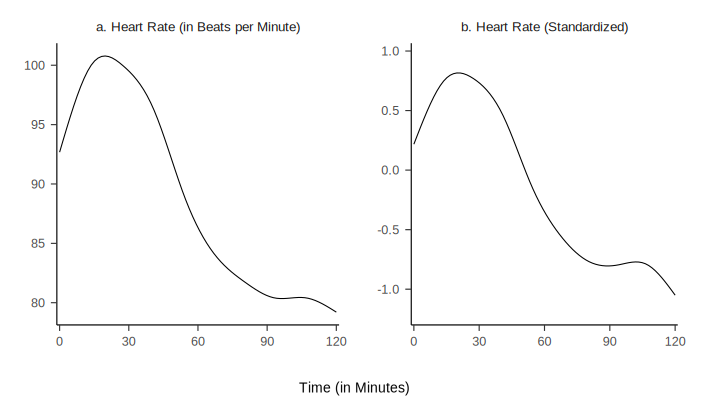
\includegraphics[width=1\textwidth]{plots_publication/loess_plot_std_unstd_new.pdf}
  \caption{Overall course of the HR with the unstandardized HR in BPM shown in Fig. 3a. and the z-standardized HR shown in Fig. 3b. for the planned 2-hour study.}
  \label{Overall course of the HR with the unstandardized HR in BPM shown in Fig. 3a. and the z-standardized HR shown in Fig. 3b. for the planned 2-hour study.}
\end{figure}

\begin{figure}[H]
  \centering
  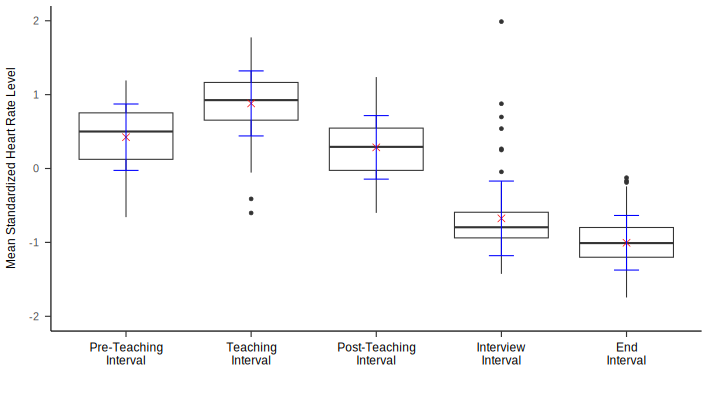
\includegraphics[width=1\textwidth]{plots_publication/box_plot.pdf}
  \caption{Distribution of the standardized heart rate means in the five intervals}
  \label{Distribution of the standardized heart rate means in the five intervals}
\end{figure}

\renewcommand{\arraystretch}{1.5}

\begin{table}[ht]
    \centering
    \begin{tabularx}{\textwidth}{lXXXXX}
        \toprule
        Interval & n\tablefootnote{All measurement points per interval for all participants. Note that the variation in $n$ stems from the variation in the number of collected data points by the fitness tracker.} & \multicolumn{2}{c}{\textit{M (SD)}} & \multicolumn{2}{c}{$p$} \\
        & & Intercept & Slope & Intercept & Slope \\
        \midrule
        (1) Pre-teaching interval & 6896 & 0.052  & 0.085*  & .57 & $<$ .05 \\
        & & (0.820) & (0.133) & & \\
        (2) Teaching interval & 7150 & 1.025* & -0.039* & $<$ .05 & $<$ .05 \\
        & & (0.690) & (0.108) & & \\
        (3) Post-teaching interval & 6664 & 0.549* & -0.060* & $<$ .05 & $<$ .05 \\
        & & (0.547) & (0.101) & & \\
        (4) Interview interval & 6287 & -0.617* & -0.022 & $<$ .05 & .006 \\
        & & (0.614) & (0.070) & & \\
        (5) End interval & 5990 & -1.004* & -0.012 & $<$ .05 & .14 \\
        & & (0.500) & (0.074) & & \\
        \bottomrule \\
        Note. * $p < .05$
    \end{tabularx}
    \caption{Descriptive statistics (n, M, SD) for the mean intercepts and the mean slopes for the five intervals.}
    \label{tab_2}
\end{table}

\renewcommand{\arraystretch}{1.5}

\begin{table}[ht]
    \centering
    \begin{tabularx}{\textwidth}{lccccc}
        \toprule
        Variable & Pre-teaching & Teaching & Post-teaching & Interview & End \\
        & interval & interval & interval & interval & interval \\
        \midrule
        Teaching Experience & $- .17/ - .27^*$ & .11/-.02 & $- .04/-.03$ & $.24^*/-.20$ & .04/.11 \\
        Disruption Appraisal & $- .01/.16$ & $- .20/.08$ & .20/$- .14$ & $- .13/.01$ & .04/.12 \\
        Confidence Appraisal & $- .10/ - .18$ & .06/.09 & .04/$- .03$ & .09/$- .19$ & $- .07/.13$ \\
        \bottomrule \\
          Note. * $p < .05$.
    \end{tabularx}
    \caption{Correlations between mean standardized HR/mean slopes and the predictor variables of teaching experience (TE), disruption appraisal (DA), and confidence appraisal (CA) for the five intervals.}
    \label{tab_3}
\end{table}

\begin{landscape}

% Set longtable to stretch the entire width of the page
\setlength{\LTleft}{0pt}
\setlength{\LTright}{0pt}

\begin{longtable}{@{\extracolsep{\fill}} p{1.8cm} p{1cm} p{1cm} p{1cm} p{1cm} p{1cm} p{1cm} p{1cm} p{1cm} p{1cm} p{1cm} p{1cm} p{1cm} p{1cm} p{1cm} p{1cm} p{1cm} @{}}

    \toprule
    & \multicolumn{4}{c}{Model 1} & \multicolumn{4}{c}{Model 2} & \multicolumn{4}{c}{Model 3} & \multicolumn{4}{c}{Model 4} \\
    \cmidrule(lr){2-5} \cmidrule(lr){6-9} \cmidrule(lr){10-13} \cmidrule(lr){14-17}
    Dependent \newline variable: & \multicolumn{16}{c}{Mean standardized HR and mean slopes} \\
    \cmidrule(lr){2-17}
    & \multicolumn{2}{c}{Mean std. HR} & \multicolumn{2}{c}{Mean slopes} & \multicolumn{2}{c}{Mean std. HR} & \multicolumn{2}{c}{Mean slopes} & \multicolumn{2}{c}{Mean std. HR} & \multicolumn{2}{c}{Mean slopes} & \multicolumn{2}{c}{Mean std. HR} & \multicolumn{2}{c}{Mean slopes} \\
    & $\beta$ (SE) & $p$ & $\beta$ (SE) & $p$ & $\beta$ (SE) & $p$ & $\beta$ (SE) & $p$ & $\beta$ (SE) & $p$ & $\beta$ (SE) & $p$ & $\beta$ (SE) & $p$ & $\beta$ (SE) & $p$ \\
    \midrule
    \endfirsthead

    \multicolumn{17}{c}{{\bfseries \tablename\ \thetable{} -- continued from previous page}} \\
    \toprule
    & \multicolumn{4}{c}{Model 1} & \multicolumn{4}{c}{Model 2} & \multicolumn{4}{c}{Model 3} & \multicolumn{4}{c}{Model 4} \\
    \cmidrule(lr){2-5} \cmidrule(lr){6-9} \cmidrule(lr){10-13} \cmidrule(lr){14-17}
    Dependent variable: & \multicolumn{16}{c}{Mean standardized HR and mean slopes} \\
    \cmidrule(lr){2-17}
    & $\beta$ (SE) & $p$ & $\beta$ (SE) & $p$ & $\beta$ (SE) & $p$ & $\beta$ (SE) & $p$ & $\beta$ (SE) & $p$ & $\beta$ (SE) & $p$ & $\beta$ (SE) & $p$ & $\beta$ (SE) & $p$ \\
    \midrule
    \endhead

    \bottomrule
    \multicolumn{17}{c}{{Continued on next page}} \\
    \endfoot

    \bottomrule
    \endlastfoot

    Pre-teaching \newline interval (I1) & & & & & & & & & & & & & & & & \\
    Teaching \newline Experience & \begin{tabular}{@{}c@{}}$-.17$\\$(.005)$\end{tabular} & $.12$ & \begin{tabular}{@{}c@{}}$-.27^*$\\$(.002)$\end{tabular} & $<.05$ & & & & & & & & & & & & \\
    R\textsuperscript{2} & $.030$ & & $.071$ & & & & & & & & & & & & & \\
    \midrule
    Teaching \newline interval (I2) & & & & & & & & & & & & & & & & \\
    Teaching \newline Experience & \begin{tabular}{@{}c@{}}$.11$\\$(.002)$\end{tabular} & $.34$ & \begin{tabular}{@{}c@{}}$-.02$\\$(.001)$\end{tabular} & $.83$ & \begin{tabular}{@{}c@{}}$.04$\\$(.005)$\end{tabular} & $.73$ & \begin{tabular}{@{}c@{}}$.01$\\$(.001)$\end{tabular} & $.96$ & \begin{tabular}{@{}c@{}}$.10$\\$(.006)$\end{tabular} & $.42$ & \begin{tabular}{@{}c@{}}$-.08$\\$(.001)$\end{tabular} & $.54$ & \begin{tabular}{@{}c@{}}$.05$\\$(.006)$\end{tabular} & $.67$ & \begin{tabular}{@{}c@{}}$-.05$\\$(.001)$\end{tabular} & $.72$ \\
    Disruption \newline Appraisal & \begin{tabular}{@{}c@{}}$-.18$\\$(.041)$\end{tabular} & $.13$ & \begin{tabular}{@{}c@{}}$.08$\\$(.010)$\end{tabular} & $.50$ & \begin{tabular}{@{}c@{}}$-.19$\\$(.042)$\end{tabular} & $.13$ & \begin{tabular}{@{}c@{}}$.12$\\$(.010)$\end{tabular} & $.34$ \\
    Confidence \newline Appraisal & \begin{tabular}{@{}c@{}}$.01$\\$(.046)$\end{tabular} & $.92$ & \begin{tabular}{@{}c@{}}$.12$\\$(.011)$\end{tabular} & $.34$ & \begin{tabular}{@{}c@{}}$-.04$\\$(.047)$\end{tabular} & $.76$ & \begin{tabular}{@{}c@{}}$.15$\\$(.012)$\end{tabular} & $.24$ \\
    R\textsuperscript{2} & $.012$ & & $.000$ & & $.040$ & & $.015$ & & $.012$ & & $.010$ & & $.042$ & & $.031$ \\
    $\Delta$ R\textsuperscript{2} & & & $.028$ & & $.015$ & & $.000$ & & $.010$ & & $.030$ & & $.031$ \\
    \midrule
    Post-teaching \newline interval (I3) & & & & & & & & & & & & & & & & \\
    Teaching \newline Experience & \begin{tabular}{@{}c@{}}$-.04$\\$(.005)$\end{tabular} & $.70$ & \begin{tabular}{@{}c@{}}$-.03$\\$(.001)$\end{tabular} & $.80$ & \begin{tabular}{@{}c@{}}$.04$\\$(.005)$\end{tabular} & $.76$ & \begin{tabular}{@{}c@{}}$-.09$\\$(.001)$\end{tabular} & $.44$ & \begin{tabular}{@{}c@{}}$-.08$\\$(.006)$\end{tabular} & $.55$ & \begin{tabular}{@{}c@{}}$-.02$\\$(.001)$\end{tabular} & $.89$ & \begin{tabular}{@{}c@{}}$-.01$\\$(.006)$\end{tabular} & $.91$ & \begin{tabular}{@{}c@{}}$-.07$\\$(.001)$\end{tabular} & $.61$ \\
    Disruption \newline Appraisal & \begin{tabular}{@{}c@{}}$.22$\\$(.040)$\end{tabular} & $.07$ & \begin{tabular}{@{}c@{}}$-.18$\\$(.009)$\end{tabular} & $.14$ & \begin{tabular}{@{}c@{}}$.25^*$\\$(.041)$\end{tabular} & $<.05$ & \begin{tabular}{@{}c@{}}$-.20$\\$(.010)$\end{tabular} & $.12$ \\
    Confidence \newline Appraisal & \begin{tabular}{@{}c@{}}$.08$\\$(.045)$\end{tabular} & $.55$ & \begin{tabular}{@{}c@{}}$-.03$\\$(.011)$\end{tabular} & $.83$ & \begin{tabular}{@{}c@{}}$.14$\\$(.046)$\end{tabular} & $.27$ & \begin{tabular}{@{}c@{}}$-.08$\\$(.011)$\end{tabular} & $.54$ \\
    R\textsuperscript{2} & $.002$ & & $.001$ & & $.043$ & & $.020$ & & $.006$ & & $.002$ & & $.058$ & & $.023$ \\
    $\Delta$ R\textsuperscript{2} & & & $.041$ & & $.019$ & & $.004$ & & $.001$ & & $.056$ & & $.022$ \\
    \midrule
    Interview \newline interval (I4) & & & & & & & & & & & & & & & & \\
    Teaching \newline Experience & \begin{tabular}{@{}c@{}}$.24^*$\\$(.006)$\end{tabular} & $<.05$ & \begin{tabular}{@{}c@{}}$-.20$\\$(.001)$\end{tabular} & $.07$ & \begin{tabular}{@{}c@{}}$.22$\\$(.006)$\end{tabular} & $.06$ & \begin{tabular}{@{}c@{}}$-.23$\\$(.001)$\end{tabular} & $.06$ & \begin{tabular}{@{}c@{}}$.25^*$\\$(.006)$\end{tabular} & $<.05$ & \begin{tabular}{@{}c@{}}$-.14$\\$(.001)$\end{tabular} & $.25$ & \begin{tabular}{@{}c@{}}$.23$\\$(.007)$\end{tabular} & $.07$ & \begin{tabular}{@{}c@{}}$-.17$\\$(.001)$\end{tabular} & $.18$ \\
    Disruption \newline Appraisal & \begin{tabular}{@{}c@{}}$-.05$\\$(.045)$\end{tabular} & $.66$ & \begin{tabular}{@{}c@{}}$-.08$\\$(.006)$\end{tabular} & $.52$ & \begin{tabular}{@{}c@{}}$-.06$\\$(.047)$\end{tabular} & $.61$ & \begin{tabular}{@{}c@{}}$-.12$\\$(.007)$\end{tabular} & $.34$ \\
    Confidence \newline Appraisal & \begin{tabular}{@{}c@{}}$-.02$\\$(.050)$\end{tabular} & $.85$ & \begin{tabular}{@{}c@{}}$-.13$\\$(.007)$\end{tabular} & $.29$ & \begin{tabular}{@{}c@{}}$-.04$\\$(.052)$\end{tabular} & $.76$ & \begin{tabular}{@{}c@{}}$-.16$\\$(.007)$\end{tabular} & $.20$ \\
    R\textsuperscript{2} & $.058$ & & $.040$ & & $.060$ & & $.050$ & & $.058$ & & $.054$ & & $.061$ & & $.069$ \\
    $\Delta$ R\textsuperscript{2} & & & $.002$ & & $.010$ & & $.000$ & & $.014$ & & $.003$ & & $.029$ \\
    \midrule
    End \newline interval (I5) & & & & & & & & & & & & & & & & \\
    Teaching \newline Experience & \begin{tabular}{@{}c@{}}$.04$\\$(.004)$\end{tabular} & $.70$ & \begin{tabular}{@{}c@{}}$.11$\\$(.001)$\end{tabular} & $.32$ & \begin{tabular}{@{}c@{}}$.07$\\$(.005)$\end{tabular} & $.58$ & \begin{tabular}{@{}c@{}}$.18$\\$(.001)$\end{tabular} & $.13$ & \begin{tabular}{@{}c@{}}$.09$\\$(.005)$\end{tabular} & $.46$ & \begin{tabular}{@{}c@{}}$.07$\\$(.001)$\end{tabular} & $.58$ & \begin{tabular}{@{}c@{}}$.10$\\$(.005)$\end{tabular} & $.43$ & \begin{tabular}{@{}c@{}}$.12$\\$(.001)$\end{tabular} & $.33$ \\
    Disruption \newline Appraisal & \begin{tabular}{@{}c@{}}$.06$\\$(.035)$\end{tabular} & $.60$ & \begin{tabular}{@{}c@{}}$.19$\\$(.007)$\end{tabular} & $.12$ & \begin{tabular}{@{}c@{}}$.04$\\$(.037)$\end{tabular} & $.76$ & \begin{tabular}{@{}c@{}}$.23$\\$(.007)$\end{tabular} & $.07$ \\
    Confidence \newline Appraisal & \begin{tabular}{@{}c@{}}$-.11$\\$(.039)$\end{tabular} & $.38$ & \begin{tabular}{@{}c@{}}$.10$\\$(.008)$\end{tabular} & $.43$ & \begin{tabular}{@{}c@{}}$-.10$\\$(.041)$\end{tabular} & $.44$ & \begin{tabular}{@{}c@{}}$.16$\\$(.008)$\end{tabular} & $.22$ \\
    R\textsuperscript{2} & $.002$ & & $.013$ & & $.005$ & & $.053$ & & $.012$ & & $.025$ & & $.013$ & & $.078$ \\
    $\Delta$ R\textsuperscript{2} & & & $.003$ & & $.040$ & & $.010$ & & $.012$ & & $.011$ & & $.065$ \\
\end{longtable}
\begin{tablenotes}
\footnotesize
\item Note. In Model 1, mean standardized HR and mean slopes were predicted only by teaching experience. In Model 2, solely disruption appraisal was added to teaching experience as a predictor. In Model 3, solely confidence appraisal was added to teaching experience as a predictor. In Model 4, all three predictors were considered in concert.
\item * $p < .05$.
\end{tablenotes}
\end{landscape}

\bibliography{r-references.bib}


\end{document}
